\chapter{Solution Approach}
Given an application-defined workload specification (i.e., query templates and a performance goal), we generate a set of workload execution strategies that can be used to execute incoming query workloads with low cost and within the application’s performance goal. Formally, our goal is to identify strategies that minimize the total cost as defined in equation \eqref{eq:1}.
Towards this end, our framework generates samples of optimal schedules (i.e., that minimize the total cost) and relies on decision tree classifiers to learn “good” strategies from these optimal solutions. 
\begin{figure}
\centering
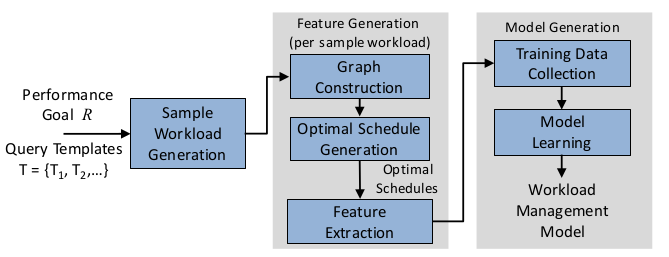
\includegraphics[width=1.0\textwidth]{generation.png}
\caption{\label{fig:generation}Generation of decision model}
\end{figure}
Our framework is depicted in Figure ~\ref{fig:generation}. Initially, we create a large number of random sample workloads, each consisting of a small number of queries drawn from the query template definitions. Our next step is to identify the optimal schedule for each of these sample workloads. To do this efficiently, we represent the problem of scheduling workloads as a graph navigation problem. On this graph, edges represent query assignment or resource provisioning decisions and the weight of each edge is equal to the cost of that decision. Hence, each path through the graph represents decisions that compose some schedule for the given workload. Finding the optimal schedule for that workload is thus reduced to finding the shortest path on this graph. Next, for each decision within an optimal schedule, we extract a set of features that characterize this decision. We then generate a training set which includes all collected features from all the optimal schedules across all sample workloads. Finally, we train a decision tree model on this training set. The learning process is executed offline and the generated models can be used during runtime on incoming workloads. The approach is discussed in detail in next chapters.
